% Options for packages loaded elsewhere
\PassOptionsToPackage{unicode}{hyperref}
\PassOptionsToPackage{hyphens}{url}
%
\documentclass[
]{article}
\usepackage{amsmath,amssymb}
\usepackage{lmodern}
\usepackage{iftex}
\ifPDFTeX
  \usepackage[T1]{fontenc}
  \usepackage[utf8]{inputenc}
  \usepackage{textcomp} % provide euro and other symbols
\else % if luatex or xetex
  \usepackage{unicode-math}
  \defaultfontfeatures{Scale=MatchLowercase}
  \defaultfontfeatures[\rmfamily]{Ligatures=TeX,Scale=1}
\fi
% Use upquote if available, for straight quotes in verbatim environments
\IfFileExists{upquote.sty}{\usepackage{upquote}}{}
\IfFileExists{microtype.sty}{% use microtype if available
  \usepackage[]{microtype}
  \UseMicrotypeSet[protrusion]{basicmath} % disable protrusion for tt fonts
}{}
\makeatletter
\@ifundefined{KOMAClassName}{% if non-KOMA class
  \IfFileExists{parskip.sty}{%
    \usepackage{parskip}
  }{% else
    \setlength{\parindent}{0pt}
    \setlength{\parskip}{6pt plus 2pt minus 1pt}}
}{% if KOMA class
  \KOMAoptions{parskip=half}}
\makeatother
\usepackage{xcolor}
\usepackage[margin=1in]{geometry}
\usepackage{color}
\usepackage{fancyvrb}
\newcommand{\VerbBar}{|}
\newcommand{\VERB}{\Verb[commandchars=\\\{\}]}
\DefineVerbatimEnvironment{Highlighting}{Verbatim}{commandchars=\\\{\}}
% Add ',fontsize=\small' for more characters per line
\usepackage{framed}
\definecolor{shadecolor}{RGB}{248,248,248}
\newenvironment{Shaded}{\begin{snugshade}}{\end{snugshade}}
\newcommand{\AlertTok}[1]{\textcolor[rgb]{0.94,0.16,0.16}{#1}}
\newcommand{\AnnotationTok}[1]{\textcolor[rgb]{0.56,0.35,0.01}{\textbf{\textit{#1}}}}
\newcommand{\AttributeTok}[1]{\textcolor[rgb]{0.77,0.63,0.00}{#1}}
\newcommand{\BaseNTok}[1]{\textcolor[rgb]{0.00,0.00,0.81}{#1}}
\newcommand{\BuiltInTok}[1]{#1}
\newcommand{\CharTok}[1]{\textcolor[rgb]{0.31,0.60,0.02}{#1}}
\newcommand{\CommentTok}[1]{\textcolor[rgb]{0.56,0.35,0.01}{\textit{#1}}}
\newcommand{\CommentVarTok}[1]{\textcolor[rgb]{0.56,0.35,0.01}{\textbf{\textit{#1}}}}
\newcommand{\ConstantTok}[1]{\textcolor[rgb]{0.00,0.00,0.00}{#1}}
\newcommand{\ControlFlowTok}[1]{\textcolor[rgb]{0.13,0.29,0.53}{\textbf{#1}}}
\newcommand{\DataTypeTok}[1]{\textcolor[rgb]{0.13,0.29,0.53}{#1}}
\newcommand{\DecValTok}[1]{\textcolor[rgb]{0.00,0.00,0.81}{#1}}
\newcommand{\DocumentationTok}[1]{\textcolor[rgb]{0.56,0.35,0.01}{\textbf{\textit{#1}}}}
\newcommand{\ErrorTok}[1]{\textcolor[rgb]{0.64,0.00,0.00}{\textbf{#1}}}
\newcommand{\ExtensionTok}[1]{#1}
\newcommand{\FloatTok}[1]{\textcolor[rgb]{0.00,0.00,0.81}{#1}}
\newcommand{\FunctionTok}[1]{\textcolor[rgb]{0.00,0.00,0.00}{#1}}
\newcommand{\ImportTok}[1]{#1}
\newcommand{\InformationTok}[1]{\textcolor[rgb]{0.56,0.35,0.01}{\textbf{\textit{#1}}}}
\newcommand{\KeywordTok}[1]{\textcolor[rgb]{0.13,0.29,0.53}{\textbf{#1}}}
\newcommand{\NormalTok}[1]{#1}
\newcommand{\OperatorTok}[1]{\textcolor[rgb]{0.81,0.36,0.00}{\textbf{#1}}}
\newcommand{\OtherTok}[1]{\textcolor[rgb]{0.56,0.35,0.01}{#1}}
\newcommand{\PreprocessorTok}[1]{\textcolor[rgb]{0.56,0.35,0.01}{\textit{#1}}}
\newcommand{\RegionMarkerTok}[1]{#1}
\newcommand{\SpecialCharTok}[1]{\textcolor[rgb]{0.00,0.00,0.00}{#1}}
\newcommand{\SpecialStringTok}[1]{\textcolor[rgb]{0.31,0.60,0.02}{#1}}
\newcommand{\StringTok}[1]{\textcolor[rgb]{0.31,0.60,0.02}{#1}}
\newcommand{\VariableTok}[1]{\textcolor[rgb]{0.00,0.00,0.00}{#1}}
\newcommand{\VerbatimStringTok}[1]{\textcolor[rgb]{0.31,0.60,0.02}{#1}}
\newcommand{\WarningTok}[1]{\textcolor[rgb]{0.56,0.35,0.01}{\textbf{\textit{#1}}}}
\usepackage{graphicx}
\makeatletter
\def\maxwidth{\ifdim\Gin@nat@width>\linewidth\linewidth\else\Gin@nat@width\fi}
\def\maxheight{\ifdim\Gin@nat@height>\textheight\textheight\else\Gin@nat@height\fi}
\makeatother
% Scale images if necessary, so that they will not overflow the page
% margins by default, and it is still possible to overwrite the defaults
% using explicit options in \includegraphics[width, height, ...]{}
\setkeys{Gin}{width=\maxwidth,height=\maxheight,keepaspectratio}
% Set default figure placement to htbp
\makeatletter
\def\fps@figure{htbp}
\makeatother
\setlength{\emergencystretch}{3em} % prevent overfull lines
\providecommand{\tightlist}{%
  \setlength{\itemsep}{0pt}\setlength{\parskip}{0pt}}
\setcounter{secnumdepth}{-\maxdimen} % remove section numbering
\ifLuaTeX
  \usepackage{selnolig}  % disable illegal ligatures
\fi
\IfFileExists{bookmark.sty}{\usepackage{bookmark}}{\usepackage{hyperref}}
\IfFileExists{xurl.sty}{\usepackage{xurl}}{} % add URL line breaks if available
\urlstyle{same} % disable monospaced font for URLs
\hypersetup{
  pdftitle={Lab 1 - Regressione Lineare in R},
  pdfauthor={Ilaria Prosdocimi},
  hidelinks,
  pdfcreator={LaTeX via pandoc}}

\title{Lab 1 - Regressione Lineare in R}
\author{Ilaria Prosdocimi}
\date{Semestre 1 - AA 2022/23}

\begin{document}
\maketitle

{
\setcounter{tocdepth}{2}
\tableofcontents
}
\begin{Shaded}
\begin{Highlighting}[]
\NormalTok{getwd()}
\end{Highlighting}
\end{Shaded}

In questo lab useremo il file che contiene informazioni sui pinguini
delle isole Palmers:

\begin{Shaded}
\begin{Highlighting}[]
\NormalTok{pengs }\OtherTok{\textless{}{-}} \FunctionTok{read.csv}\NormalTok{(}\StringTok{"../data/penguins.csv"}\NormalTok{)}
\FunctionTok{summary}\NormalTok{(pengs)}
\end{Highlighting}
\end{Shaded}

\begin{verbatim}
##    species             island          bill_length_mm  bill_depth_mm  
##  Length:344         Length:344         Min.   :32.10   Min.   :13.10  
##  Class :character   Class :character   1st Qu.:39.23   1st Qu.:15.60  
##  Mode  :character   Mode  :character   Median :44.45   Median :17.30  
##                                        Mean   :43.92   Mean   :17.15  
##                                        3rd Qu.:48.50   3rd Qu.:18.70  
##                                        Max.   :59.60   Max.   :21.50  
##                                        NA's   :2       NA's   :2      
##  flipper_length_mm  body_mass_g       sex                 year     
##  Min.   :172.0     Min.   :2700   Length:344         Min.   :2007  
##  1st Qu.:190.0     1st Qu.:3550   Class :character   1st Qu.:2007  
##  Median :197.0     Median :4050   Mode  :character   Median :2008  
##  Mean   :200.9     Mean   :4202                      Mean   :2008  
##  3rd Qu.:213.0     3rd Qu.:4750                      3rd Qu.:2009  
##  Max.   :231.0     Max.   :6300                      Max.   :2009  
##  NA's   :2         NA's   :2
\end{verbatim}

\begin{Shaded}
\begin{Highlighting}[]
\DocumentationTok{\#\# eliminiamo le righe con valori mancanti (non è sempre una buona idea) }
\NormalTok{pengs }\OtherTok{\textless{}{-}} \FunctionTok{na.omit}\NormalTok{(pengs)}
\FunctionTok{nrow}\NormalTok{(pengs)}
\end{Highlighting}
\end{Shaded}

\begin{verbatim}
## [1] 333
\end{verbatim}

Il primo modello in esame prevede di stimare come la lunghezza della
pinna di un pinguino (\texttt{flipper\_length\_mm}) varia in funzione
della massa \texttt{body\_mass\_g}.

\begin{Shaded}
\begin{Highlighting}[]
\FunctionTok{plot}\NormalTok{(pengs[,}\FunctionTok{c}\NormalTok{(}\StringTok{"flipper\_length\_mm"}\NormalTok{,}\StringTok{"body\_mass\_g"}\NormalTok{)])}
\end{Highlighting}
\end{Shaded}

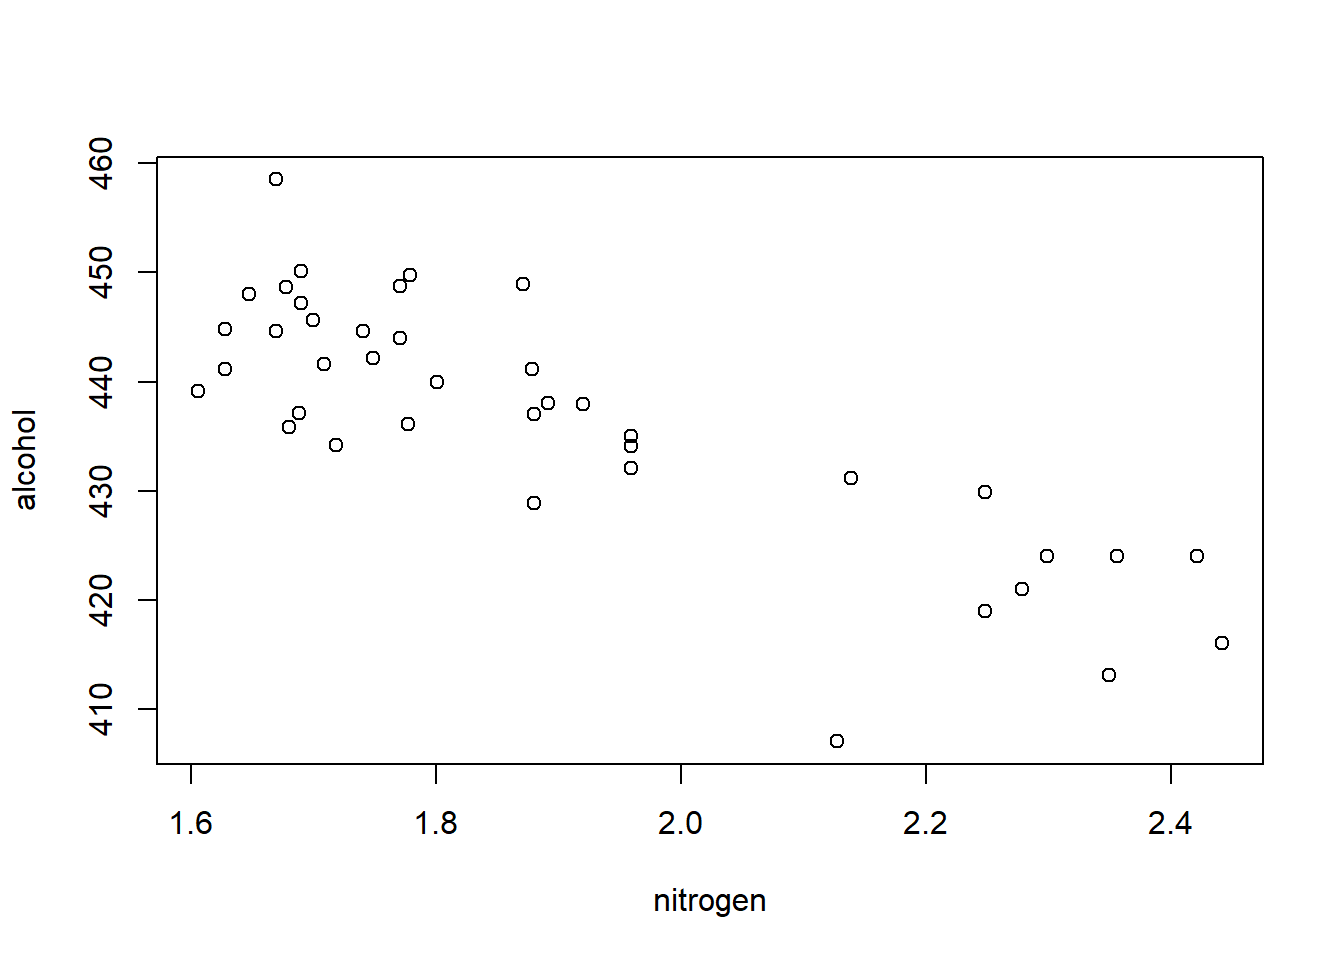
\includegraphics{lab01_files/figure-latex/unnamed-chunk-2-1.pdf}

Possiamo usare gli stimatori plug-in ed ottenre:

\[\hat{\beta}_1 = \frac{c_{XY}}{s^2_{X}} =  r_{XY} \frac{s_{Y}}{s_{X}},\quad \mbox{and} \quad \hat{\beta}_0 = \overline{y}-\hat{\beta}_1 \overline{x}  \]

\begin{Shaded}
\begin{Highlighting}[]
\NormalTok{rxy }\OtherTok{\textless{}{-}} \FunctionTok{cor}\NormalTok{(pengs}\SpecialCharTok{$}\NormalTok{flipper\_length\_mm, pengs}\SpecialCharTok{$}\NormalTok{body\_mass\_g)}
\NormalTok{sx }\OtherTok{\textless{}{-}} \FunctionTok{sd}\NormalTok{(pengs}\SpecialCharTok{$}\NormalTok{body\_mass\_g); sy }\OtherTok{\textless{}{-}} \FunctionTok{sd}\NormalTok{(pengs}\SpecialCharTok{$}\NormalTok{flipper\_length\_mm)}
\NormalTok{mx }\OtherTok{\textless{}{-}} \FunctionTok{mean}\NormalTok{(pengs}\SpecialCharTok{$}\NormalTok{body\_mass\_g)}
\NormalTok{my }\OtherTok{\textless{}{-}} \FunctionTok{mean}\NormalTok{(pengs}\SpecialCharTok{$}\NormalTok{flipper\_length\_mm)}
\NormalTok{beta1\_hat }\OtherTok{\textless{}{-}}\NormalTok{ rxy}\SpecialCharTok{*}\NormalTok{sy}\SpecialCharTok{/}\NormalTok{sx}
\NormalTok{beta0\_hat }\OtherTok{\textless{}{-}}\NormalTok{ my }\SpecialCharTok{{-}}\NormalTok{ beta1\_hat }\SpecialCharTok{*}\NormalTok{ mx}
\FunctionTok{c}\NormalTok{(beta0\_hat, beta1\_hat)}
\end{Highlighting}
\end{Shaded}

\begin{verbatim}
## [1] 137.03962089   0.01519526
\end{verbatim}

Oppure, più realisticamente possiamo usare le funzioni già presenti in
R.

\hypertarget{modelli-lineari-in-r}{%
\section{Modelli lineari in R}\label{modelli-lineari-in-r}}

La principale funzione da usare per stimare modelli lineari in R è
\texttt{lm} - (si veda \texttt{help(lm)}).

I primo argomento di \texttt{lm} è \texttt{formula}: con questo
argomento si specifica a sinistra di una tilde quale è la variabile
risposta e a destra della tilde quale sia il predittore del modello (o i
predittori):

\begin{Shaded}
\begin{Highlighting}[]
\NormalTok{fit }\OtherTok{\textless{}{-}} \FunctionTok{lm}\NormalTok{(flipper\_length\_mm}\SpecialCharTok{\textasciitilde{}}\NormalTok{body\_mass\_g, }\AttributeTok{data =}\NormalTok{ pengs)}
\end{Highlighting}
\end{Shaded}

Possiamo a questo punto \emph{stampare} \texttt{fit} per avere
informazioni di base:

\begin{Shaded}
\begin{Highlighting}[]
\NormalTok{fit }\DocumentationTok{\#\# in R this corresponds to print(fit)}
\end{Highlighting}
\end{Shaded}

\begin{verbatim}
## 
## Call:
## lm(formula = flipper_length_mm ~ body_mass_g, data = pengs)
## 
## Coefficients:
## (Intercept)  body_mass_g  
##    137.0396       0.0152
\end{verbatim}

La stampa mostra i valori dei coefficienti di un modello lineare
semplice: questi sono i valori stimati tramite least square. Possiamo
ottenere i valori dei parametri anche con

\begin{Shaded}
\begin{Highlighting}[]
\FunctionTok{coef}\NormalTok{(fit)}
\end{Highlighting}
\end{Shaded}

\begin{verbatim}
##  (Intercept)  body_mass_g 
## 137.03962089   0.01519526
\end{verbatim}

Vi sono infatti una serie di funzioni che possiamo applicare all'oggetto
\texttt{fit} che ha classe \texttt{lm}:

\begin{Shaded}
\begin{Highlighting}[]
\FunctionTok{class}\NormalTok{(fit)}
\end{Highlighting}
\end{Shaded}

\begin{verbatim}
## [1] "lm"
\end{verbatim}

Tra le funzioni più utili ci sono per esempio \texttt{fitted}, che
deriva i valori stimati per le \(y_i\) (quindi valuta la funzione
\(\beta_0 + \beta_1 x_i\) prendendo le stime dei minimi quadrati per
\(\beta_0\) e \(\beta_1\)):

\begin{Shaded}
\begin{Highlighting}[]
\FunctionTok{head}\NormalTok{(}\FunctionTok{coef}\NormalTok{(fit)[}\DecValTok{1}\NormalTok{]}\SpecialCharTok{+}\FunctionTok{coef}\NormalTok{(fit)[}\DecValTok{2}\NormalTok{]}\SpecialCharTok{*}\NormalTok{pengs}\SpecialCharTok{$}\NormalTok{body\_mass\_g)}
\end{Highlighting}
\end{Shaded}

\begin{verbatim}
## [1] 194.0219 194.7816 186.4242 189.4633 192.5023 192.1225
\end{verbatim}

\begin{Shaded}
\begin{Highlighting}[]
\FunctionTok{head}\NormalTok{(}\FunctionTok{fitted}\NormalTok{(fit))}
\end{Highlighting}
\end{Shaded}

\begin{verbatim}
##        1        2        3        5        6        7 
## 194.0219 194.7816 186.4242 189.4633 192.5023 192.1225
\end{verbatim}

Vedremo poi che una funzione molto utile è \texttt{summary}

\begin{Shaded}
\begin{Highlighting}[]
\FunctionTok{summary}\NormalTok{(fit)}
\end{Highlighting}
\end{Shaded}

\begin{verbatim}
## 
## Call:
## lm(formula = flipper_length_mm ~ body_mass_g, data = pengs)
## 
## Residuals:
##     Min      1Q  Median      3Q     Max 
## -23.698  -4.983   1.056   5.101  13.933 
## 
## Coefficients:
##              Estimate Std. Error t value Pr(>|t|)    
## (Intercept) 1.370e+02  1.999e+00   68.56   <2e-16 ***
## body_mass_g 1.520e-02  4.667e-04   32.56   <2e-16 ***
## ---
## Signif. codes:  0 '***' 0.001 '**' 0.01 '*' 0.05 '.' 0.1 ' ' 1
## 
## Residual standard error: 6.847 on 331 degrees of freedom
## Multiple R-squared:  0.7621, Adjusted R-squared:  0.7614 
## F-statistic:  1060 on 1 and 331 DF,  p-value: < 2.2e-16
\end{verbatim}

che stampa molte informazioni: vedremo nel corso le varie parti
dell'output.

Notiamo che è presente il valore stimato di \(\sigma^2\), la varianza
della variabile casuale che descrive l'errore del modello
(\(\varepsilon\)):

\[s_e^2 = \frac{1}{n}\sum_{i=1}^{n-2} (y_i - \hat{y}_i)\]

\begin{Shaded}
\begin{Highlighting}[]
\FunctionTok{summary}\NormalTok{(fit)}\SpecialCharTok{$}\NormalTok{sigma}
\end{Highlighting}
\end{Shaded}

\begin{verbatim}
## [1] 6.84662
\end{verbatim}

\begin{Shaded}
\begin{Highlighting}[]
\FunctionTok{sqrt}\NormalTok{(}\FunctionTok{sum}\NormalTok{((pengs}\SpecialCharTok{$}\NormalTok{flipper\_length\_mm  }\SpecialCharTok{{-}} \FunctionTok{fitted}\NormalTok{(fit))}\SpecialCharTok{\^{}}\DecValTok{2}\NormalTok{)}\SpecialCharTok{/}\NormalTok{(}\FunctionTok{nrow}\NormalTok{(pengs)}\SpecialCharTok{{-}}\DecValTok{2}\NormalTok{))}
\end{Highlighting}
\end{Shaded}

\begin{verbatim}
## [1] 6.84662
\end{verbatim}

La stima di \(\sigma\) viene usata per stimare l'incertezza della stima
dei coefficienti del modello:

\[Var[\widehat{\beta}_0]= sigma_e^2\left[\frac{1}{n} + \frac{\overline{x}^2}{n s^2_X}\right]\]
\[Var[\widehat{\beta}_1] = \frac{ sigma_e^2}{n s^2_X}\]

\begin{Shaded}
\begin{Highlighting}[]
\NormalTok{se }\OtherTok{\textless{}{-}} \FunctionTok{summary}\NormalTok{(fit)}\SpecialCharTok{$}\NormalTok{sigma}
\NormalTok{n }\OtherTok{\textless{}{-}} \FunctionTok{nrow}\NormalTok{(pengs)}
\NormalTok{s2x }\OtherTok{\textless{}{-}} \FunctionTok{sum}\NormalTok{((pengs}\SpecialCharTok{$}\NormalTok{body\_mass\_g }\SpecialCharTok{{-}} \FunctionTok{mean}\NormalTok{(pengs}\SpecialCharTok{$}\NormalTok{body\_mass\_g))}\SpecialCharTok{\^{}}\DecValTok{2}\NormalTok{)}\SpecialCharTok{/}\NormalTok{n}
\FunctionTok{c}\NormalTok{(se }\SpecialCharTok{*} \FunctionTok{sqrt}\NormalTok{(}\DecValTok{1}\SpecialCharTok{/}\NormalTok{n }\SpecialCharTok{+} \FunctionTok{mean}\NormalTok{(pengs}\SpecialCharTok{$}\NormalTok{body\_mass\_g)}\SpecialCharTok{\^{}}\DecValTok{2}\SpecialCharTok{/}\NormalTok{(n }\SpecialCharTok{*}\NormalTok{ s2x)), se }\SpecialCharTok{*} \FunctionTok{sqrt}\NormalTok{(}\DecValTok{1}\SpecialCharTok{/}\NormalTok{(n }\SpecialCharTok{*}\NormalTok{ s2x)))}
\end{Highlighting}
\end{Shaded}

\begin{verbatim}
## [1] 1.9987694290 0.0004666539
\end{verbatim}

\begin{Shaded}
\begin{Highlighting}[]
\FunctionTok{summary}\NormalTok{(fit)}\SpecialCharTok{$}\NormalTok{coef[,}\DecValTok{2}\NormalTok{]}
\end{Highlighting}
\end{Shaded}

\begin{verbatim}
##  (Intercept)  body_mass_g 
## 1.9987694290 0.0004666539
\end{verbatim}

\textbf{Esercizio}

Cosa succede alla variabilità della stima dei coefficienti se si usa
come variabile esplicativa una nuova variabile

\begin{Shaded}
\begin{Highlighting}[]
\NormalTok{pengs}\SpecialCharTok{$}\NormalTok{mass\_minus\_4000 }\OtherTok{\textless{}{-}}\NormalTok{ pengs}\SpecialCharTok{$}\NormalTok{body\_mass\_g }\SpecialCharTok{{-}} \DecValTok{4000}
\end{Highlighting}
\end{Shaded}

E cosa succede invece se il peso viene espresso in grammi:

\begin{Shaded}
\begin{Highlighting}[]
\NormalTok{pengs}\SpecialCharTok{$}\NormalTok{body\_mass\_Kg }\OtherTok{\textless{}{-}}\NormalTok{ pengs}\SpecialCharTok{$}\NormalTok{body\_mass\_g}\SpecialCharTok{/}\DecValTok{1000}
\end{Highlighting}
\end{Shaded}

Infine, cosa cambia invece quando si cambia anche la variabile risposta,
per esempio esprimendo il valori in cm

\begin{Shaded}
\begin{Highlighting}[]
\NormalTok{pengs}\SpecialCharTok{$}\NormalTok{bill\_length\_cm }\OtherTok{\textless{}{-}}\NormalTok{ pengs}\SpecialCharTok{$}\NormalTok{bill\_length\_mm}\SpecialCharTok{*}\DecValTok{10}
\end{Highlighting}
\end{Shaded}

Anche il valore di \(R^2\) è presente nell'output:

\begin{Shaded}
\begin{Highlighting}[]
\FunctionTok{summary}\NormalTok{(fit)}\SpecialCharTok{$}\NormalTok{r.squared}
\end{Highlighting}
\end{Shaded}

\begin{verbatim}
## [1] 0.7620922
\end{verbatim}

\begin{Shaded}
\begin{Highlighting}[]
\DocumentationTok{\#\# SSreg/SStot}
\FunctionTok{sum}\NormalTok{((}\FunctionTok{fitted}\NormalTok{(fit) }\SpecialCharTok{{-}} \FunctionTok{mean}\NormalTok{(pengs}\SpecialCharTok{$}\NormalTok{flipper\_length\_mm))}\SpecialCharTok{\^{}}\DecValTok{2}\NormalTok{)}\SpecialCharTok{/}\FunctionTok{sum}\NormalTok{((pengs}\SpecialCharTok{$}\NormalTok{flipper\_length\_mm  }\SpecialCharTok{{-}} \FunctionTok{mean}\NormalTok{(pengs}\SpecialCharTok{$}\NormalTok{flipper\_length\_mm ))}\SpecialCharTok{\^{}}\DecValTok{2}\NormalTok{)}
\end{Highlighting}
\end{Shaded}

\begin{verbatim}
## [1] 0.7620922
\end{verbatim}

\begin{Shaded}
\begin{Highlighting}[]
\CommentTok{\# 1{-} SSres/SStot }
\DecValTok{1} \SpecialCharTok{{-}} \FunctionTok{sum}\NormalTok{((pengs}\SpecialCharTok{$}\NormalTok{flipper\_length\_mm  }\SpecialCharTok{{-}} \FunctionTok{fitted}\NormalTok{(fit))}\SpecialCharTok{\^{}}\DecValTok{2}\NormalTok{)}\SpecialCharTok{/}\FunctionTok{sum}\NormalTok{((pengs}\SpecialCharTok{$}\NormalTok{flipper\_length\_mm  }\SpecialCharTok{{-}} \FunctionTok{mean}\NormalTok{(pengs}\SpecialCharTok{$}\NormalTok{flipper\_length\_mm ))}\SpecialCharTok{\^{}}\DecValTok{2}\NormalTok{)}
\end{Highlighting}
\end{Shaded}

\begin{verbatim}
## [1] 0.7620922
\end{verbatim}

Infine la funzione \texttt{residuals} restituisce i residui del modello:

\begin{Shaded}
\begin{Highlighting}[]
\FunctionTok{head}\NormalTok{(}\FunctionTok{residuals}\NormalTok{(fit))}
\end{Highlighting}
\end{Shaded}

\begin{verbatim}
##          1          2          3          5          6          7 
## -13.021864  -8.781627   8.575768   3.536715  -2.502337 -11.122456
\end{verbatim}

\begin{Shaded}
\begin{Highlighting}[]
\FunctionTok{head}\NormalTok{((pengs}\SpecialCharTok{$}\NormalTok{flipper\_length\_mm }\SpecialCharTok{{-}} \FunctionTok{fitted}\NormalTok{(fit)))}
\end{Highlighting}
\end{Shaded}

\begin{verbatim}
##          1          2          3          5          6          7 
## -13.021864  -8.781627   8.575768   3.536715  -2.502337 -11.122456
\end{verbatim}

Ricordiamo alcune proprietà dei residui che derivano dalle equazioni di
stima (estimating equations):

\begin{Shaded}
\begin{Highlighting}[]
\CommentTok{\# mean of residuals is null }
\FunctionTok{mean}\NormalTok{(}\FunctionTok{residuals}\NormalTok{(fit))}
\end{Highlighting}
\end{Shaded}

\begin{verbatim}
## [1] -1.653217e-15
\end{verbatim}

\begin{Shaded}
\begin{Highlighting}[]
\CommentTok{\# no correlation with X {-} }
\CommentTok{\# this does not mean that there is not relationship left between X and the residuals }
\FunctionTok{cor}\NormalTok{(}\FunctionTok{residuals}\NormalTok{(fit), pengs}\SpecialCharTok{$}\NormalTok{body\_mass\_g)}
\end{Highlighting}
\end{Shaded}

\begin{verbatim}
## [1] 1.668496e-16
\end{verbatim}

\hypertarget{predizione-ed-incertezza}{%
\section{Predizione ed incertezza}\label{predizione-ed-incertezza}}

Ora che il modello è stato stimato, possiamo usarlo per predirre nuovi
valori di \(Y|X=x\): mentre la funzione \texttt{fitted} restituisce i
valori di \(Y\) stimati \emph{per le x osservate nel campione}
(\(\hat{y_i}\)), possiamo usare la funzione \texttt{predict} per
valutare la funzione in dei diversi valori di \(x\) (di default però la
funzione predice i valori nel campione osservato):

\begin{Shaded}
\begin{Highlighting}[]
\FunctionTok{head}\NormalTok{(}\FunctionTok{fitted}\NormalTok{(fit))}
\end{Highlighting}
\end{Shaded}

\begin{verbatim}
##        1        2        3        5        6        7 
## 194.0219 194.7816 186.4242 189.4633 192.5023 192.1225
\end{verbatim}

\begin{Shaded}
\begin{Highlighting}[]
\FunctionTok{head}\NormalTok{(}\FunctionTok{predict}\NormalTok{(fit))}
\end{Highlighting}
\end{Shaded}

\begin{verbatim}
##        1        2        3        5        6        7 
## 194.0219 194.7816 186.4242 189.4633 192.5023 192.1225
\end{verbatim}

\begin{Shaded}
\begin{Highlighting}[]
\FunctionTok{predict}\NormalTok{(fit, }\AttributeTok{newdata =} \FunctionTok{data.frame}\NormalTok{(}\AttributeTok{body\_mass\_g =} \FunctionTok{c}\NormalTok{(}\DecValTok{3500}\NormalTok{,}\DecValTok{4000}\NormalTok{,}\DecValTok{4700}\NormalTok{)))}
\end{Highlighting}
\end{Shaded}

\begin{verbatim}
##        1        2        3 
## 190.2230 197.8207 208.4574
\end{verbatim}

\begin{Shaded}
\begin{Highlighting}[]
\FunctionTok{coef}\NormalTok{(fit)[}\DecValTok{1}\NormalTok{]}\SpecialCharTok{+}\FunctionTok{coef}\NormalTok{(fit)[}\DecValTok{2}\NormalTok{] }\SpecialCharTok{*} \DecValTok{3500}\NormalTok{; }\FunctionTok{coef}\NormalTok{(fit)[}\DecValTok{1}\NormalTok{]}\SpecialCharTok{+}\FunctionTok{coef}\NormalTok{(fit)[}\DecValTok{2}\NormalTok{] }\SpecialCharTok{*} \DecValTok{4000}\NormalTok{; }\FunctionTok{coef}\NormalTok{(fit)[}\DecValTok{1}\NormalTok{]}\SpecialCharTok{+}\FunctionTok{coef}\NormalTok{(fit)[}\DecValTok{2}\NormalTok{] }\SpecialCharTok{*} \DecValTok{4700}
\end{Highlighting}
\end{Shaded}

\begin{verbatim}
## (Intercept) 
##     190.223
\end{verbatim}

\begin{verbatim}
## (Intercept) 
##    197.8207
\end{verbatim}

\begin{verbatim}
## (Intercept) 
##    208.4574
\end{verbatim}

\begin{Shaded}
\begin{Highlighting}[]
\DocumentationTok{\#\# what does the slope value mean? }
\FunctionTok{predict}\NormalTok{(fit, }\AttributeTok{newdata =} \FunctionTok{data.frame}\NormalTok{(}\AttributeTok{body\_mass\_g =} \DecValTok{3501}\NormalTok{)) }\SpecialCharTok{{-}} \FunctionTok{predict}\NormalTok{(fit, }\AttributeTok{newdata =} \FunctionTok{data.frame}\NormalTok{(}\AttributeTok{body\_mass\_g =} \DecValTok{3500}\NormalTok{))}
\end{Highlighting}
\end{Shaded}

\begin{verbatim}
##          1 
## 0.01519526
\end{verbatim}

\begin{Shaded}
\begin{Highlighting}[]
\FunctionTok{coef}\NormalTok{(fit)[}\DecValTok{2}\NormalTok{]}
\end{Highlighting}
\end{Shaded}

\begin{verbatim}
## body_mass_g 
##  0.01519526
\end{verbatim}

\begin{Shaded}
\begin{Highlighting}[]
\DocumentationTok{\#\# what does the intercept value mean? }
\FunctionTok{predict}\NormalTok{(fit, }\AttributeTok{newdata =} \FunctionTok{data.frame}\NormalTok{(}\AttributeTok{body\_mass\_g =} \DecValTok{0}\NormalTok{))}
\end{Highlighting}
\end{Shaded}

\begin{verbatim}
##        1 
## 137.0396
\end{verbatim}

\begin{Shaded}
\begin{Highlighting}[]
\FunctionTok{coef}\NormalTok{(fit)[}\DecValTok{1}\NormalTok{]}
\end{Highlighting}
\end{Shaded}

\begin{verbatim}
## (Intercept) 
##    137.0396
\end{verbatim}

La funzione \texttt{predict} inoltre permette di specificare se
desideriamo ottenere qualche informazione sull'incertezza della stima:
in particolare si possono ottenere i valori della deviazione standard
attorno ad \(E[m(x)]\), derivati come:
\[\hat{SE}[\hat{m}(x)] = s_e\sqrt{\frac{1}{n}+\frac{(x-\bar{x})^2}{\sum_{i = 1}^n(x_i-\overline{x})^2}}\]
dove \(s_e\) è la deviazione standard dell'errore:

\begin{Shaded}
\begin{Highlighting}[]
\NormalTok{sepengs }\OtherTok{\textless{}{-}} \FunctionTok{sqrt}\NormalTok{(}\FunctionTok{sum}\NormalTok{((pengs}\SpecialCharTok{$}\NormalTok{flipper\_length\_mm}\SpecialCharTok{{-}}\NormalTok{fit}\SpecialCharTok{$}\NormalTok{fitted.values)}\SpecialCharTok{\^{}}\DecValTok{2}\NormalTok{)}\SpecialCharTok{/}\NormalTok{(}\FunctionTok{nrow}\NormalTok{(pengs)}\SpecialCharTok{{-}}\DecValTok{2}\NormalTok{))}
\NormalTok{sepengs}
\end{Highlighting}
\end{Shaded}

\begin{verbatim}
## [1] 6.84662
\end{verbatim}

Il valore della deviazione standard attorno al valore atteso di
\(Y|X=x\) dipende da \(x\), il valore in cui valutiamo la funzione
\(m(x)\):

\begin{Shaded}
\begin{Highlighting}[]
\NormalTok{n }\OtherTok{\textless{}{-}} \FunctionTok{nrow}\NormalTok{(pengs)}
\CommentTok{\# error for x = 4000}
\NormalTok{sepengs }\SpecialCharTok{*} \FunctionTok{sqrt}\NormalTok{((}\DecValTok{1}\SpecialCharTok{/}\NormalTok{n }\SpecialCharTok{+}\NormalTok{ ((}\DecValTok{4000}\SpecialCharTok{{-}}\FunctionTok{mean}\NormalTok{(pengs}\SpecialCharTok{$}\NormalTok{body\_mass\_g))}\SpecialCharTok{\^{}}\DecValTok{2}\NormalTok{)}\SpecialCharTok{/}\FunctionTok{sum}\NormalTok{((pengs}\SpecialCharTok{$}\NormalTok{body\_mass\_g}\SpecialCharTok{{-}}\FunctionTok{mean}\NormalTok{(pengs}\SpecialCharTok{$}\NormalTok{body\_mass\_g))}\SpecialCharTok{\^{}}\DecValTok{2}\NormalTok{)))}
\end{Highlighting}
\end{Shaded}

\begin{verbatim}
## [1] 0.3874346
\end{verbatim}

\begin{Shaded}
\begin{Highlighting}[]
\NormalTok{(pred1 }\OtherTok{\textless{}{-}} \FunctionTok{predict}\NormalTok{(fit, }\AttributeTok{newdata =} \FunctionTok{data.frame}\NormalTok{(}\AttributeTok{body\_mass\_g =} \DecValTok{4000}\NormalTok{), }\AttributeTok{se.fit =} \ConstantTok{TRUE}\NormalTok{))}
\end{Highlighting}
\end{Shaded}

\begin{verbatim}
## $fit
##        1 
## 197.8207 
## 
## $se.fit
## [1] 0.3874346
## 
## $df
## [1] 331
## 
## $residual.scale
## [1] 6.84662
\end{verbatim}

\begin{Shaded}
\begin{Highlighting}[]
\NormalTok{pred1}\SpecialCharTok{$}\NormalTok{se.fit}
\end{Highlighting}
\end{Shaded}

\begin{verbatim}
## [1] 0.3874346
\end{verbatim}

\begin{Shaded}
\begin{Highlighting}[]
\CommentTok{\# error for x = 5000}
\NormalTok{sepengs }\SpecialCharTok{*} \FunctionTok{sqrt}\NormalTok{((}\DecValTok{1}\SpecialCharTok{/}\NormalTok{n }\SpecialCharTok{+}\NormalTok{ ((}\DecValTok{5000}\SpecialCharTok{{-}}\FunctionTok{mean}\NormalTok{(pengs}\SpecialCharTok{$}\NormalTok{body\_mass\_g))}\SpecialCharTok{\^{}}\DecValTok{2}\NormalTok{)}\SpecialCharTok{/}\FunctionTok{sum}\NormalTok{((pengs}\SpecialCharTok{$}\NormalTok{body\_mass\_g}\SpecialCharTok{{-}}\FunctionTok{mean}\NormalTok{(pengs}\SpecialCharTok{$}\NormalTok{body\_mass\_g))}\SpecialCharTok{\^{}}\DecValTok{2}\NormalTok{)))}
\end{Highlighting}
\end{Shaded}

\begin{verbatim}
## [1] 0.5269645
\end{verbatim}

\begin{Shaded}
\begin{Highlighting}[]
\NormalTok{pred2 }\OtherTok{\textless{}{-}} \FunctionTok{predict}\NormalTok{(fit, }\AttributeTok{newdata =} \FunctionTok{data.frame}\NormalTok{(}\AttributeTok{body\_mass\_g =} \DecValTok{5000}\NormalTok{), }\AttributeTok{se.fit =} \ConstantTok{TRUE}\NormalTok{)}
\NormalTok{pred2}\SpecialCharTok{$}\NormalTok{se.fit}
\end{Highlighting}
\end{Shaded}

\begin{verbatim}
## [1] 0.5269645
\end{verbatim}

Possiamo derivare l'incertezza attorno a diverse predizioni:

\begin{Shaded}
\begin{Highlighting}[]
\FunctionTok{mean}\NormalTok{(pengs}\SpecialCharTok{$}\NormalTok{body\_mass\_g)}
\end{Highlighting}
\end{Shaded}

\begin{verbatim}
## [1] 4207.057
\end{verbatim}

\begin{Shaded}
\begin{Highlighting}[]
\FunctionTok{predict}\NormalTok{(fit, }\AttributeTok{newdata =} \FunctionTok{data.frame}\NormalTok{(}\AttributeTok{body\_mass\_g =} \FunctionTok{c}\NormalTok{(}\DecValTok{1500}\NormalTok{,}\DecValTok{4200}\NormalTok{,}\DecValTok{5000}\NormalTok{,}\DecValTok{8000}\NormalTok{)), }\AttributeTok{se.fit =} \ConstantTok{TRUE}\NormalTok{)}\SpecialCharTok{$}\NormalTok{se.fit}
\end{Highlighting}
\end{Shaded}

\begin{verbatim}
##         1         2         3         4 
## 1.3177982 0.3752069 0.5269645 1.8093203
\end{verbatim}

Si nota come vi sia incertezza sempre maggiore più il valore di \(x\) è
distante da \(\overline{x}\).

\hypertarget{verifica-delle-assunzioni-del-modello}{%
\section{Verifica delle assunzioni del
modello}\label{verifica-delle-assunzioni-del-modello}}

La stima dei minimi quadrati si basa su alcune assunzioni non troppo
stringenti: si assume che la relazione tra \(X\) ed \(Y\) possa essere
approssimata da una relazione lineare. Altre assunzioni sono necessarie
per poter derivare proprietà essenziali degli stimatori, in particolare
si assume che gli errori del modello siano indipendenti e identicamente
distribuiti con varianza costante.

Sebbene non sia possibile osservare gli errori del modello, possiamo
osservare i residui, cioè la differenza tra valori osservati e stimati
(dal modello) della variabile risposta: \(r_i = (y_i-\hat{y}_i)\). In R
si possono ottenere i valori di \(r_i\) con \texttt{residuals}:

\begin{Shaded}
\begin{Highlighting}[]
\FunctionTok{head}\NormalTok{(}\FunctionTok{residuals}\NormalTok{(fit))}
\end{Highlighting}
\end{Shaded}

\begin{verbatim}
##          1          2          3          5          6          7 
## -13.021864  -8.781627   8.575768   3.536715  -2.502337 -11.122456
\end{verbatim}

\begin{Shaded}
\begin{Highlighting}[]
\CommentTok{\# by hand}
\FunctionTok{head}\NormalTok{(pengs}\SpecialCharTok{$}\NormalTok{flipper\_length\_mm}\SpecialCharTok{{-}}\FunctionTok{fitted}\NormalTok{(fit))}
\end{Highlighting}
\end{Shaded}

\begin{verbatim}
##          1          2          3          5          6          7 
## -13.021864  -8.781627   8.575768   3.536715  -2.502337 -11.122456
\end{verbatim}

\begin{Shaded}
\begin{Highlighting}[]
\DocumentationTok{\#\# another option is }
\FunctionTok{head}\NormalTok{(fit}\SpecialCharTok{$}\NormalTok{residuals)}
\end{Highlighting}
\end{Shaded}

\begin{verbatim}
##          1          2          3          5          6          7 
## -13.021864  -8.781627   8.575768   3.536715  -2.502337 -11.122456
\end{verbatim}

L'assunzione di indipendenza è difficile da testare, ma dato che ogni
osservazione è derivata da un pinguino diverso è probabile che le
osservazioni siano indipendenti (ma cosa succede se per esempio c'è un
effetto della colonia sulla relazione di interesse e noi campioniamo
pinguini solo da una colonia?). Per verificare che la varianza sia
costante possiamo invece guardare un grafico di \(x_i\) VS \(r_i\) e
\(\hat{y}_i\) VS \(r_i\):

\begin{Shaded}
\begin{Highlighting}[]
\FunctionTok{par}\NormalTok{(}\AttributeTok{mfrow=}\FunctionTok{c}\NormalTok{(}\DecValTok{1}\NormalTok{,}\DecValTok{2}\NormalTok{), }\AttributeTok{pch=}\DecValTok{16}\NormalTok{,}\AttributeTok{bty=}\StringTok{"l"}\NormalTok{)}
\FunctionTok{plot}\NormalTok{(pengs}\SpecialCharTok{$}\NormalTok{body\_mass\_g, }\FunctionTok{residuals}\NormalTok{(fit))}
\FunctionTok{plot}\NormalTok{(}\FunctionTok{fitted}\NormalTok{(fit), }\FunctionTok{residuals}\NormalTok{(fit))}
\end{Highlighting}
\end{Shaded}

\includegraphics{lab01_files/figure-latex/homeSched-1.pdf}

Non ci sono forti segnali di varianza non costante, ma è presente una
qualche struttura nei grafici.

R inoltre produce di default una serie di utili grafici basati sui
residui quando si usa la funzione \texttt{plot} su un oggetto di classe
\texttt{lm}:

\begin{Shaded}
\begin{Highlighting}[]
\FunctionTok{par}\NormalTok{(}\AttributeTok{mfrow=}\FunctionTok{c}\NormalTok{(}\DecValTok{2}\NormalTok{,}\DecValTok{2}\NormalTok{))}
\FunctionTok{plot}\NormalTok{(fit)}
\end{Highlighting}
\end{Shaded}

\includegraphics{lab01_files/figure-latex/residChecks-1.pdf}

Vedremo più in dettaglio questi grafici nelle prossime lezioni.

Sebbene sia stato mostrato come il modello di regressione lineare sia
relativamente robusto ad alcune deviazioni dal modello - la stima dei
parametri si basa sulle assunzioni specificate: se queste assunzioni non
sono riscontrabili nei dati si corre il rischio di fare un inferenza non
affidabile. è sempre raccomandabile verificare che le assunzioni del
modello siano soddisfatte prima di utilizzare un modello per fare
predizioni e prendere decisioni.

\hypertarget{verifiche-della-teoria-tramite-simulazione}{%
\section{Verifiche della teoria tramite
simulazione}\label{verifiche-della-teoria-tramite-simulazione}}

La simulazione è un approccio molto utile per indagare come si
comportano i vari metodi di stima e per verificare in maniera empirica
come si comportano gli stimatori. Il creare una procedura di simulazione
dei dati per altro aiuta molto a capire in profondità quali sia il
processo sotteso alla generazione dei dati che viene ipotizzato dal
modello.

Valutiamo quindi alcune proprietà degli stimatori tramite la simulazione
di dati le cui caratteristiche possiamo controllare, per esmepio
valutiamo la proprietà di non-distorsione e le formule derivate per la
varianza degli stimatori:

\begin{Shaded}
\begin{Highlighting}[]
\FunctionTok{set.seed}\NormalTok{(}\DecValTok{324}\NormalTok{) }\CommentTok{\# per riproducibilità }
\NormalTok{n }\OtherTok{\textless{}{-}} \DecValTok{100} 
\NormalTok{x }\OtherTok{\textless{}{-}} \FunctionTok{runif}\NormalTok{(n, }\SpecialCharTok{{-}}\DecValTok{1}\NormalTok{, }\DecValTok{1}\NormalTok{)}
\DocumentationTok{\#\# le x sono fissate}
\DocumentationTok{\#\# i veri valori dei coefficienti del modello }
\NormalTok{b0 }\OtherTok{\textless{}{-}} \DecValTok{1}\NormalTok{; b1 }\OtherTok{\textless{}{-}} \DecValTok{2}

\CommentTok{\# una possibile realizzazione del modello }
\NormalTok{epsilon }\OtherTok{\textless{}{-}} \FunctionTok{rexp}\NormalTok{(n,}\DecValTok{1}\NormalTok{)}\SpecialCharTok{{-}}\DecValTok{1} \DocumentationTok{\#\# errori a media 0 }
\CommentTok{\# alcune alternative }
\CommentTok{\# epsilon \textless{}{-} runif(n,{-}1,1) \#\# errori a media 0 }
\CommentTok{\# epsilon \textless{}{-} runif(n,{-}3,3) \#\# errori a media 0 }
\CommentTok{\# epsilon \textless{}{-} rgamma(n,shape = 4, scale = 2){-}8  \#\# errori a media 0 }
\CommentTok{\# epsilon \textless{}{-} rexp(n,4){-}1/4 \#\# errori a media 0 }
\CommentTok{\# epsilon \textless{}{-} rnorm(n,0,2) \#\# errori a media 0 }
\NormalTok{y }\OtherTok{\textless{}{-}}\NormalTok{ b0 }\SpecialCharTok{+}\NormalTok{ b1 }\SpecialCharTok{*}\NormalTok{ x }\SpecialCharTok{+}\NormalTok{ epsilon}
\FunctionTok{coef}\NormalTok{(}\FunctionTok{lm}\NormalTok{(y}\SpecialCharTok{\textasciitilde{}}\NormalTok{x)) }\CommentTok{\# close enough }
\end{Highlighting}
\end{Shaded}

\begin{verbatim}
## (Intercept)           x 
##    1.045610    1.960217
\end{verbatim}

\begin{Shaded}
\begin{Highlighting}[]
\DocumentationTok{\#\# do this 1000 time }
\NormalTok{generate\_get\_betas }\OtherTok{\textless{}{-}} \ControlFlowTok{function}\NormalTok{(bs, epsilonpar, x)\{}
\NormalTok{  ytemp }\OtherTok{\textless{}{-}}\NormalTok{ b0 }\SpecialCharTok{+}\NormalTok{ b1 }\SpecialCharTok{*}\NormalTok{ x }\SpecialCharTok{+}\NormalTok{ (}\FunctionTok{rexp}\NormalTok{(}\FunctionTok{length}\NormalTok{(x),epsilonpar)}\SpecialCharTok{{-}}\DecValTok{1}\SpecialCharTok{/}\NormalTok{epsilonpar)}
  \FunctionTok{lm}\NormalTok{(ytemp}\SpecialCharTok{\textasciitilde{}}\NormalTok{x)}\SpecialCharTok{$}\NormalTok{coef}
\NormalTok{\}}
\FunctionTok{generate\_get\_betas}\NormalTok{(}\AttributeTok{bs=} \FunctionTok{c}\NormalTok{(b0,b1), }\AttributeTok{epsilonpar =} \DecValTok{1}\NormalTok{, }\AttributeTok{x =}\NormalTok{ x)}
\end{Highlighting}
\end{Shaded}

\begin{verbatim}
## (Intercept)           x 
##   0.9384214   2.3639180
\end{verbatim}

\begin{Shaded}
\begin{Highlighting}[]
\NormalTok{out }\OtherTok{\textless{}{-}} \FunctionTok{replicate}\NormalTok{(}\DecValTok{1000}\NormalTok{, }\FunctionTok{generate\_get\_betas}\NormalTok{(}\AttributeTok{bs=} \FunctionTok{c}\NormalTok{(b0,b1), }\AttributeTok{epsilonpar =} \DecValTok{1}\NormalTok{, }\AttributeTok{x =}\NormalTok{ x))}
\FunctionTok{par}\NormalTok{(}\AttributeTok{mfrow=}\FunctionTok{c}\NormalTok{(}\DecValTok{1}\NormalTok{,}\DecValTok{2}\NormalTok{))}
\FunctionTok{hist}\NormalTok{(out[}\DecValTok{1}\NormalTok{,]);}\FunctionTok{hist}\NormalTok{(out[}\DecValTok{2}\NormalTok{,])}
\end{Highlighting}
\end{Shaded}

\includegraphics{lab01_files/figure-latex/unnamed-chunk-20-1.pdf}

\begin{Shaded}
\begin{Highlighting}[]
\CommentTok{\# che forma hanno questi istogrammi? }
\CommentTok{\# unbiased }
\FunctionTok{rowMeans}\NormalTok{(out)}
\end{Highlighting}
\end{Shaded}

\begin{verbatim}
## (Intercept)           x 
##   0.9992941   2.0088404
\end{verbatim}

\begin{Shaded}
\begin{Highlighting}[]
\CommentTok{\# variability}
\FunctionTok{apply}\NormalTok{(out,}\DecValTok{1}\NormalTok{,sd)}
\end{Highlighting}
\end{Shaded}

\begin{verbatim}
## (Intercept)           x 
##   0.1016541   0.1863891
\end{verbatim}

\begin{Shaded}
\begin{Highlighting}[]
\NormalTok{se }\OtherTok{\textless{}{-}} \DecValTok{1} \CommentTok{\# V[Y] = 1/lambda\^{}2, when Y \textasciitilde{} exp(1)}
\NormalTok{s2x }\OtherTok{\textless{}{-}} \FunctionTok{sum}\NormalTok{((x}\SpecialCharTok{{-}}\FunctionTok{mean}\NormalTok{(x))}\SpecialCharTok{\^{}}\DecValTok{2}\NormalTok{)}\SpecialCharTok{/}\NormalTok{n}
\FunctionTok{c}\NormalTok{(se }\SpecialCharTok{*} \FunctionTok{sqrt}\NormalTok{(}\DecValTok{1}\SpecialCharTok{/}\NormalTok{n }\SpecialCharTok{+} \FunctionTok{mean}\NormalTok{(x)}\SpecialCharTok{\^{}}\DecValTok{2}\SpecialCharTok{/}\NormalTok{(n }\SpecialCharTok{*}\NormalTok{ s2x)), se }\SpecialCharTok{*} \FunctionTok{sqrt}\NormalTok{(}\DecValTok{1}\SpecialCharTok{/}\NormalTok{(n }\SpecialCharTok{*}\NormalTok{ s2x)))}
\end{Highlighting}
\end{Shaded}

\begin{verbatim}
## [1] 0.1000168 0.1837407
\end{verbatim}

\begin{Shaded}
\begin{Highlighting}[]
\DocumentationTok{\#\# change the variability of the error }
\NormalTok{out2 }\OtherTok{\textless{}{-}} \FunctionTok{replicate}\NormalTok{(}\DecValTok{1000}\NormalTok{, }\FunctionTok{generate\_get\_betas}\NormalTok{(}\AttributeTok{bs=} \FunctionTok{c}\NormalTok{(b0,b1), }\AttributeTok{epsilonpar =} \FloatTok{0.45}\NormalTok{, }\AttributeTok{x =}\NormalTok{ x))}
\FunctionTok{apply}\NormalTok{(out2,}\DecValTok{1}\NormalTok{,sd)}
\end{Highlighting}
\end{Shaded}

\begin{verbatim}
## (Intercept)           x 
##   0.2148624   0.4025549
\end{verbatim}

\begin{Shaded}
\begin{Highlighting}[]
\CommentTok{\# still unbiased }
\FunctionTok{apply}\NormalTok{(out2,}\DecValTok{1}\NormalTok{,mean)}
\end{Highlighting}
\end{Shaded}

\begin{verbatim}
## (Intercept)           x 
##   0.9936145   2.0086663
\end{verbatim}

\end{document}
